


\tikzset{every picture/.style={line width=0.75pt}} %set default line width to 0.75pt        

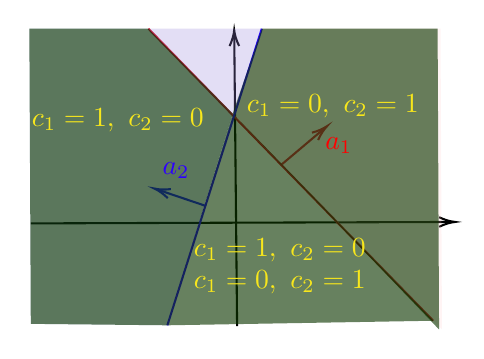
\begin{tikzpicture}[x=0.75pt,y=0.75pt,yscale=-0.7,xscale=0.7]
	%uncomment if require: \path (0,300); %set diagram left start at 0, and has height of 300
	
	%Straight Lines [id:da043120004745246465] 
	\draw    (18.43,141) -- (308.43,140.01) ;
	\draw [shift={(310.43,140)}, rotate = 179.8] [color={rgb, 255:red, 0; green, 0; blue, 0 }  ][line width=0.75]    (10.93,-3.29) .. controls (6.95,-1.4) and (3.31,-0.3) .. (0,0) .. controls (3.31,0.3) and (6.95,1.4) .. (10.93,3.29)   ;
	%Straight Lines [id:da10089229777665709] 
	\draw    (160.43,211.71) -- (158.45,10) ;
	\draw [shift={(158.43,8)}, rotate = 89.44] [color={rgb, 255:red, 0; green, 0; blue, 0 }  ][line width=0.75]    (10.93,-3.29) .. controls (6.95,-1.4) and (3.31,-0.3) .. (0,0) .. controls (3.31,0.3) and (6.95,1.4) .. (10.93,3.29)   ;
	%Straight Lines [id:da7268273424354579] 
	\draw [color={rgb, 255:red, 208; green, 2; blue, 27 }  ,draw opacity=1 ]   (190.43,101) -- (220.9,75.29) ;
	\draw [shift={(222.43,74)}, rotate = 139.84] [color={rgb, 255:red, 208; green, 2; blue, 27 }  ,draw opacity=1 ][line width=0.75]    (10.93,-3.29) .. controls (6.95,-1.4) and (3.31,-0.3) .. (0,0) .. controls (3.31,0.3) and (6.95,1.4) .. (10.93,3.29)   ;
	%Straight Lines [id:da5256799633351579] 
	\draw [color={rgb, 255:red, 208; green, 2; blue, 27 }  ,draw opacity=1 ]   (99.43,7) -- (295.43,208) ;
	%Shape: Polygon [id:ds16795660112353028] 
	\draw  [draw opacity=0][fill={rgb, 255:red, 253; green, 195; blue, 195 }  ,fill opacity=0.19 ] (300.43,7) -- (301.43,214) -- (99.43,7) -- cycle ;
	%Shape: Polygon [id:ds657177688701895] 
	\draw  [draw opacity=0][fill={rgb, 255:red, 1; green, 44; blue, 255 }  ,fill opacity=0.11 ] (177.43,7) -- (112.43,211.14) -- (18.43,210.14) -- (17.43,7) -- cycle ;
	%Straight Lines [id:da523733379699233] 
	\draw [color={rgb, 255:red, 22; green, 20; blue, 255 }  ,draw opacity=1 ]   (138.93,129) -- (105.32,117.64) ;
	\draw [shift={(103.43,117)}, rotate = 18.68] [color={rgb, 255:red, 22; green, 20; blue, 255 }  ,draw opacity=1 ][line width=0.75]    (10.93,-3.29) .. controls (6.95,-1.4) and (3.31,-0.3) .. (0,0) .. controls (3.31,0.3) and (6.95,1.4) .. (10.93,3.29)   ;
	%Straight Lines [id:da5166718561288546] 
	\draw [color={rgb, 255:red, 34; green, 0; blue, 255 }  ,draw opacity=1 ]   (177.43,7) -- (112.43,211.14) ;
	%Shape: Polygon [id:ds9146954261231561] 
	\draw  [draw opacity=0][fill={rgb, 255:red, 14; green, 55; blue, 1 }  ,fill opacity=0.64 ] (99.43,7) -- (157.43,65.43) -- (148.58,94.07) -- (112.43,211.14) -- (18.43,210.14) -- (17.43,7) -- cycle ;
	%Shape: Polygon [id:ds7825723532393902] 
	\draw  [draw opacity=0][fill={rgb, 255:red, 14; green, 55; blue, 1 }  ,fill opacity=0.63 ] (298.43,7) -- (298.84,92.02) -- (299.43,214) -- (157.43,65.43) -- (177.43,7) -- cycle ;
	%Shape: Polygon [id:ds09269151620752769] 
	\draw  [draw opacity=0][fill={rgb, 255:red, 14; green, 55; blue, 1 }  ,fill opacity=0.63 ] (295.43,208) -- (112.43,211.14) -- (157.43,65.43) -- cycle ;
	
	% Text Node
	\draw (219,80) node [anchor=north west][inner sep=0.75pt]  [color={rgb, 255:red, 255; green, 0; blue, 0 }  ,opacity=1 ] [align=left] {$\displaystyle a_{1}$};
	% Text Node
	\draw (107,97) node [anchor=north west][inner sep=0.75pt]  [color={rgb, 255:red, 46; green, 0; blue, 255 }  ,opacity=1 ] [align=left] {$\displaystyle a_{2}$};
	% Text Node
	\draw (165,50) node [anchor=north west][inner sep=0.75pt]  [color={rgb, 255:red, 248; green, 231; blue, 28 }  ,opacity=1 ] [align=left] {$\displaystyle c_{1} =0,\ c_{2} =1$};
	% Text Node
	\draw (17,60) node [anchor=north west][inner sep=0.75pt]  [color={rgb, 255:red, 248; green, 231; blue, 28 }  ,opacity=1 ] [align=left] {$\displaystyle c_{1} =1,\ c_{2} =0$};
	% Text Node
	\draw (128.51,149.6) node [anchor=north west][inner sep=0.75pt]  [color={rgb, 255:red, 248; green, 231; blue, 28 }  ,opacity=1 ] [align=left] {$\displaystyle c_{1} =1,\ c_{2} =0$};
	% Text Node
	\draw (128.51,171.6) node [anchor=north west][inner sep=0.75pt]  [color={rgb, 255:red, 248; green, 231; blue, 28 }  ,opacity=1 ] [align=left] {$\displaystyle c_{1} =0,\ c_{2} =1$};
	
	
\end{tikzpicture}
